
% --------------------------------
\section{Sprint 1}

\subsection*{Summary}
Previous sprint 0 focused on setting up the tools and getting familiarized with the group and the project and as such sprint 1 was focused on building a programming foundation to work on and to have clear project requirements.

\subsection*{Deliverables}
Product increment for sprint 1 was written high level and low level requirements, functional and non-functional requirements, use case diagram and user stories. In terms of programming, SDM, RDM, AM and main navigation layout were implemented.


\subsection*{Sprint Planning}
The sprint goal is to implement the major modules: AM, SDM, RDM and navigation layout.
From our Backlog we added all the tasks that needed to be done for our Sprint goals.
Planning poker was used for sprint planning.
\begin{figure}[H]
    \centering
    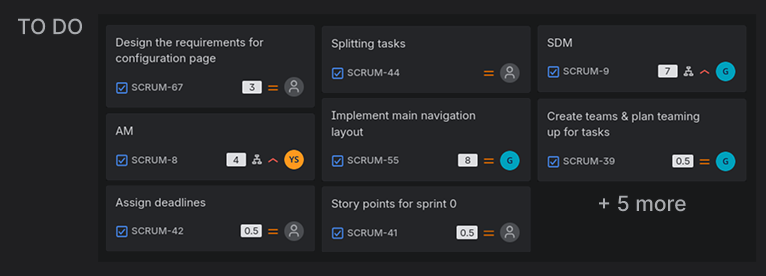
\includegraphics[width=1.0\textwidth]{Figures/Sprint/Sprint1Planning.png}
    \caption{Overview of the Jira board at the start of Sprint 1}
    \label{fig:sprint-1-planning}
\end{figure}

\subsection*{Sprint Review}
When the sprint ended, almost every single task got completed, except just one task that was not completed because we found out it was not needed. Story points estimates from sprint planning were not realistic. Furthermore, code reviews took a considerable amount of time and slowed the progress more than expected.
\begin{figure}[H]
    \centering
    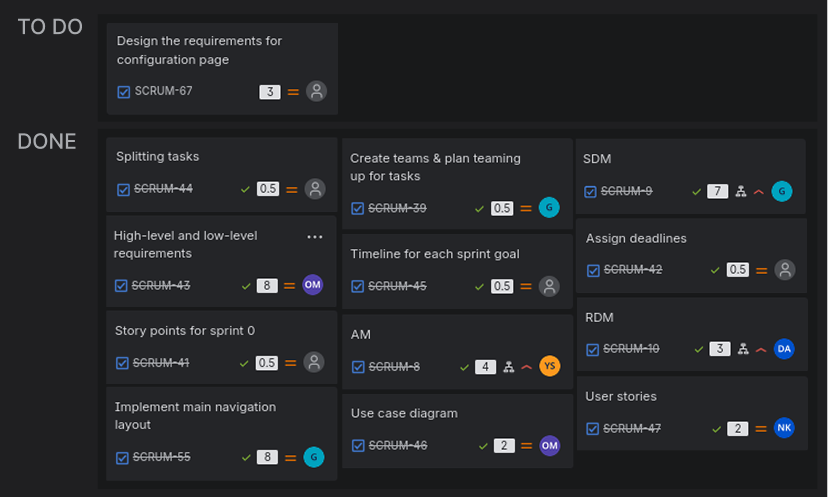
\includegraphics[width=1.0\textwidth]{Figures/Sprint/Sprint1Review.png}
    \caption{Overview of the Jira board at the end of Sprint 1}
    \label{fig:sprint-1-planning}
\end{figure}

\subsection*{Sprint Retrospective}
We did not overcommit, as we managed to deliver what was planned. Moreover, we created a solution of using an online Excalidraw canvas for decision-making to be more transparent and to encourage everyone to share their ideas. Lastly, we integrated reviews which is great for awareness and transparency, despite it taking more time.\par

We had issues with Jira's features and assignment of tasks. We have wanted to assign more than one team member for the task in Jira by using team assignment feature. However, the team assigned did not show up for the task on the board - it was only visible when previewing details of the task. Furthermore, subtasks are not easy to distribute and splitting tasks requires a lot of effort due to interdependecies, and there is no ability to assign someone to review the tasks.\par

Our team's story point estimate units did not match the reality, as tasks took about twice as long as expected. Therefore, there was not as much progress in the first week of the sprint. Moreover, members updated the Jira board with delay.\par

Distribution and assigning tasks during the Sprint Planning also came with some issues. Some tasks were assigned to people without asking them about it first. There was also some uneven distribution of tasks based on our story points, but in reality the estimates were not as accurate.\par

For the next sprint, we want to improve our task assigning both in person and in Jira. For the in-person  assigning, we want to have more discussion on what each task is about and how it can be completed. Additionally, we will focus on assigning tasks formed as questions not statements, so that people do not feel forced to do tasks. On Jira, we will use labels to assign pairs as well as reviewers. The tasks will also have better descriptions so they are clear.\par

Moreover, we want to improve the progression of tasks. As tasks take longer time to complete than expected, we want to have higher transparency with why it is happening. Therefore, we will have better questions during the stand-ups:
\begin{center}
"In fact progressing as estimated, what is in the way of the progress? Be specific."
"What was your time allocation for the task since the last meeting?"
\end{center}

\subsection*{Reflections and Conflicts}
The sprint goal was reached and tasks progressed very well. As for the conflicts, for about the first week of the sprint team engagement was relatively low and team members left unheard and their opinions ignored as they were feeling pressured and sometimes were directed to pick specific tasks. This was very prominent during time crunch situations where there was not enough time to do the tasks. In the middle of the sprint, the issue was resolved by having a shared online Excalidraw canvas during in-person meetings where tasks were listed for the session. This reduced time pressure to allocate a person for the task, team members were able to voluntarily pick tasks knowing what is needed to do and as such team engagement and working environment improved. It worked well enough that online Excalidraw canvas usage was even further expanded in the later sprints for in-person meetings.

% --------------------------------
\section{Sprint 2}
Comming...
%\subsection*{Summary}

%\subsection*{Deliverables}

%\subsection*{Sprint Planning}

%\subsection*{Sprint Review}

%\subsection*{Sprint Retrospective}

%\subsection*{Reflections and Conflicts}

% --------------------------------
\section{Sprint 3}

\subsection*{Summary}
The main focus of Sprint 3 was to finish Scenario 1 for the Optimizer. Additionally, parts of backend and frontend were finalized with general connections established. For better convenience, export of the optimization results from RDM was implemented using JSON instead of CSV. 

\subsection*{Deliverables}
Delivered product increment contained Scenario 1 Optimizer implementation, frontend and backend for Production Units page and additional expansion for RDM export.

\subsection*{Sprint Planning}
The sprint goal is to implement the connection between backend and frontend parts, implementing export from RDM. The main goal is to reach Scenario 1. The Sprint consisted of leftovers that weren’t finished in the last Sprint.
\begin{figure}[H]
    \centering
    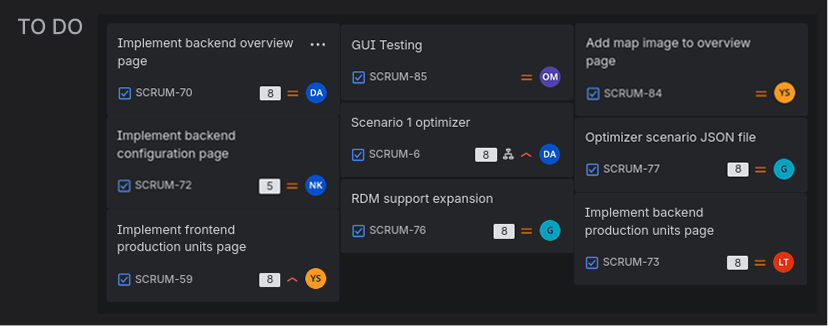
\includegraphics[width=1.0\textwidth]{Figures/Sprint/Sprint3Planning.png}
    \caption{Overview of the Jira board at the start of Sprint 3}
    \label{fig:sprint-1-planning}
\end{figure}
\subsection*{Sprint Review}
The outcome of the Sprint is quite mixed. Compared to the last Sprints we didn’t finish as many tasks. This could be a result of the distribution of tasks between members, some of which are not as experienced as others, as well as the over reliance of dependencies of other tasks.
\begin{figure}[H]
    \centering
    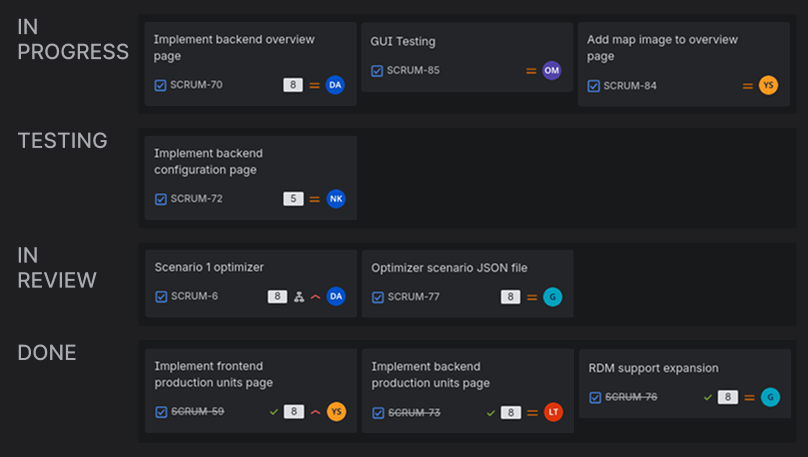
\includegraphics[width=1.0\textwidth]{Figures/Sprint/Sprint3Review.png}
    \caption{Overview of the Jira board at the end of Sprint 3}
    \label{fig:sprint-1-planning}
\end{figure}
\subsection*{Sprint Retrospective}


\subsection*{Reflections and Conflicts}
A lot of the tasks were accumulated from the end of the previous sprint, and due to the easter break overlap with one of the meetings the sprint planning was a bit more rushed. Missed deadlines could be the result of bad task distribution and not addressing equally each of the members capabilities due to less developed communication practices throughout previous sprints.\par
Although the sprint ceremonies were subject to scheduling difficulties, with more confusion as to which format to use being raised by late absence notices to in-person meetings, the results of this sprint show more transparency, communication improvements, more elaborate attempts to collaborate on resolving arising impediments. 


% --------------------------------
\section{Sprint 4}

\subsection*{Summary}
The sprint goal for this sprint was set to finalize the implementation of Scenario 2, improve the visualization of the application, and to begin working on the report. 

\subsection*{Deliverables}
The product increment during this sprint included merging the production unit page with the configuration page, finishing all backend implementation for the UI, improving the optimizer, and adding layered charts and heat grid map to the overview page.

\subsection*{Sprint Planning}
For the Sprint Planning in Sprint 4, we decided to try a new technique for assigning tasks. Everyone pre-estimated the amount of time they expected to have for the project during the two weeks, as we expected it to make the members feel more obligated to complete their tasks. After playing Planning Poker, all members selected their tasks on Jira based on their own work estimation and the corresponding story points on the tickets. The Sprint Backlog contained a few tasks from the previous sprint that were in the final stages and were completed in between our sprints, therefore we started with tickets in the done column (see Figure 3.5).
\begin{figure}[H]
    \centering
    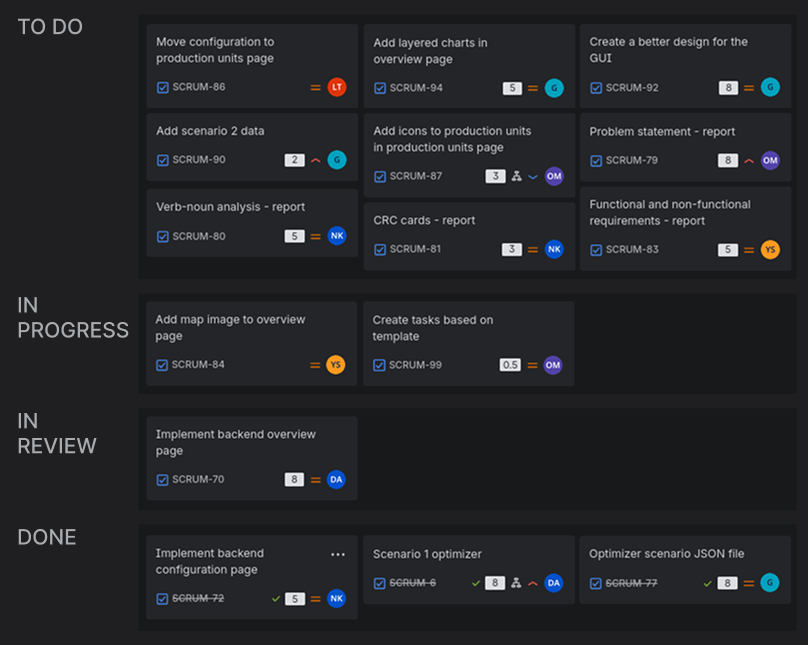
\includegraphics[width=1.0\textwidth]{Figures/Sprint/Sprint4Planning.png}
    \caption{Overview of the Jira board at the start of Sprint 4}
    \label{fig:sprint-1-planning}
\end{figure}
\subsection*{Sprint Review}
At the end of the sprint, most of the tasks were completed or in review (see Figure 3.6), with two tasks in progress and only one not started. The increment of the product did not fully satisfy the sprint goal, however we progressed a lot towards finishing the application. The Sprint 4 demonstration was moved to a later date, therefore we did not receive feedback from the stakeholders at the end of the sprint.
\begin{figure}[H]
    \centering
    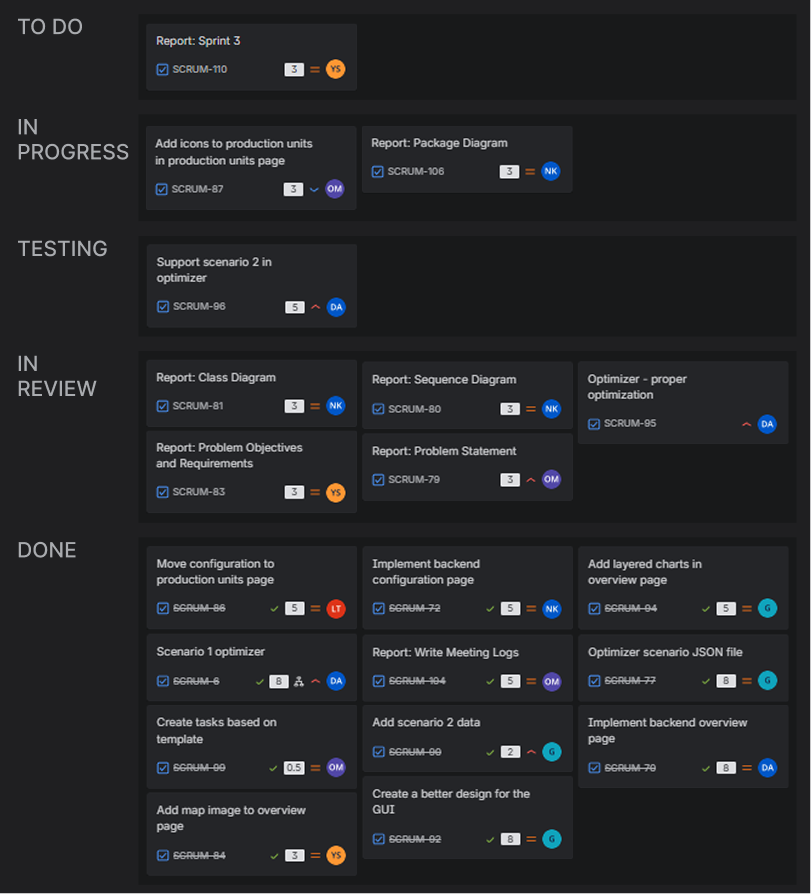
\includegraphics[width=1.0\textwidth]{Figures/Sprint/Sprint4Review.png}
    \caption{Overview of the Jira board at the end of Sprint 4}
    \label{fig:sprint-1-planning}
\end{figure}
\subsection*{Sprint Retrospective}
The Sprint Retrospective started with each member writing what worked well and what did not on our Excalidraw board, of which summary can be found in the meeting logs in the Appendix \ref{appendix:meetinglogs}. Everyone agreed that the tasks are progressing fairly well, and that implementation of more frequent communication over text messages is working. However, the issue of poor attendance was brought up. It was common that the meetings had only three to four members attending. Combined with people often getting late, the meetings seemed like they were optional and this created some discouragement, as the communication around the attendance was also quite poor.

\subsection*{Reflections and Conflicts}
To resolve the issues, we first identified the reason behind team members getting late or being absent, which turned out to be an issue with oversleeping. We came up with a solution to move the time of the meeting to a later hour to see if that will improve the attendance. Moreover, during the discussion another issue was found. Some members felt that the ending of the meetings is not clear enough, and to solve it we decided to have the end more clear.

% --------------------------------
\section{Sprint 5}

\subsection*{Summary}
During this sprint we have improved the optimizer by adding new Scenario 2 features such as support for emissions and consumptions, and handling of negative prices. The UI was also improved and the codebase was refactored to better support multiple scenarios and data handling. Additionally, we worked on the report by updating sections and handled ticket and pull request reviews to support overall project quality. 

\subsection*{Deliverables}
At the end of the sprint, we have delivered an improved optimizer with Scenario 2 features, a refined UI with better data and scenario support, and a refactored codebase supporting multiple scenarios. In addition, updated documentation and report sections, along with improved diagrams and reviewed pull requests, were completed.

\subsection*{Sprint Planning}
The sprint goal is to work on different parts of the report, including the sprint implementation, technical architecture, abstract, Scrum implementation, problem statement, diagrams, and the problem objectives and requirements. Additionally, some coding tasks were assigned, such as GUI testing and supporting implementation-related improvements. Overall, the focus is on completing both documentation and technical components to ensure consistency and final integration of the project.
\begin{figure}[H]
    \centering
    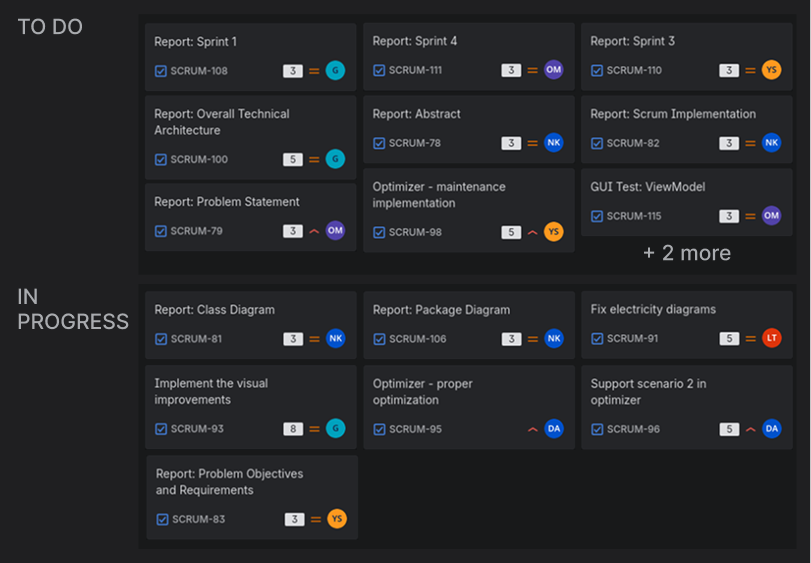
\includegraphics[width=1.0\textwidth]{Figures/Sprint/Sprint5Planning.png}
    \caption{Overview of the Jira board at the start of Sprint 5}
    \label{fig:sprint-1-planning}
\end{figure}

\subsection*{Sprint Review}
The sprint ended with most of the planned tasks completed, showing solid progress from the team. However, several tickets got stuck in the review stage, which slowed down the overall workflow. In addition, code review and validation took longer than expected, creating a bottleneck that delayed the final integration of some features. Despite these challenges, the team delivered most of the intended functionality.
\begin{figure}[H]
    \centering
    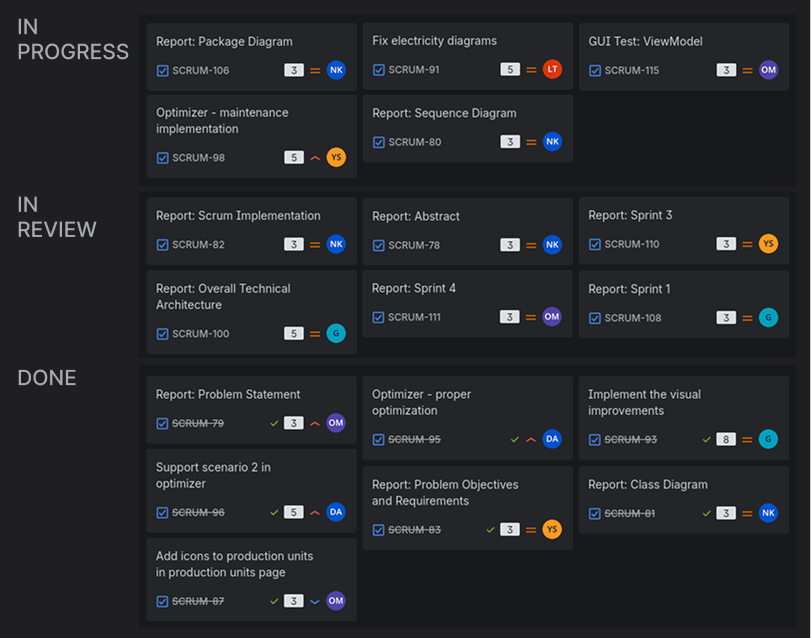
\includegraphics[width=1.0\textwidth]{Figures/Sprint/Sprint5Review.png}
    \caption{Overview of the Jira board at the end of Sprint 5}
    \label{fig:sprint-1-planning}
\end{figure}

\subsection*{Sprint Retrospective}
Communication about the tasks seems to have improved and the progression is going well. The members have started to give more elaborate answers to questions and are voicing their opinions more. Lastly, the workload was adjusted to the scheduled Math 2 exam.\par
The sprint progress was slower due to external factors such as the Math 2 exam, a slightly reduced availability due to AOP homework and other communal issues. Additionally, absences from meetings influenced progress. Notifications of absence were often sent very late, which caused organizational issues. Meetings were not always rescheduled when key participants could not attend. The group contract, which requires attendance and at least one-day advance notice of absence, was not consistently respected or enforced. Half of the team members did not meet the estimated workload defined during sprint planning by a significant margin. A large number of tasks accumulated in review and were repeatedly moved between “In Review” and “In Progress,” causing delays. This issue was further worsened by slow review activity and insufficient follow-up. As a result some tickets from the previous sprint remained in the review cycle and were not completed during this sprint. Additionally, there were inconsistencies in expectations regarding hybrid meetings and short-notice changes, which further affected coordination and planning. Although team communication has improved overall, some members still occasionally forget to inform the group about absences or meeting arrangements, which contributed to coordination issues. During one of the meetings, attendance was split between online and on-site participants, which highlighted the lack of a consistent approach to hybrid meetings.\par
The attendance issue is planned to be solved by requiring team members to send a message in the group one day before the meeting, confirming whether they can attend in person at a specified time and location or, if not, whether they can attend online. This approach accounts for the possibility of late notifications about online only attendance and allows the team to prepare for hybrid meetings in advance. If a significant number of team members are unable to attend, the meeting should be rescheduled. Regarding the review process, team members will be reminded that, as previously agreed, participation in code review is required from everyone to ensure consistent workflow and progress tracking. 

\subsection*{Reflections and Conflicts}
Communication and engagement improved, and the workload was adjusted for the Math 2 exam. However, progress was slowed by attendance issues, late notifications, and tasks getting stuck in review or not being completed from the previous sprint. Coordination was also affected by inconsistent meeting arrangements and expectations. For the next sprint, we will enforce earlier attendance confirmation, improve planning for hybrid meetings, reschedule when necessary, and set clearer deadlines for reviews to improve flow and completion rate.

% --------------------------------
\section{Sprint 6}
Comming...
%\subsection*{Summary}

%\subsection*{Deliverables}

%\subsection*{Sprint Planning}

%\subsection*{Sprint Review}

%\subsection*{Sprint Retrospective}

%\subsection*{Reflections and Conflicts}
